\documentclass[11pt]{aghdpl}
% \documentclass[en,11pt]{aghdpl}  % praca w języku angielskim

% Lista wszystkich języków stanowiących języki pozycji bibliograficznych użytych w pracy.
% (Zgodnie z zasadami tworzenia bibliografii każda pozycja powinna zostać utworzona zgodnie z zasadami języka, w którym dana publikacja została napisana.)
\usepackage[english,polish]{babel}

% Użyj polskiego łamania wyrazów (zamiast domyślnego angielskiego).
\usepackage{polski}

\usepackage[utf8]{inputenc}

% dodatkowe pakiety

\usepackage{mathtools}
\usepackage{amsfonts}
\usepackage{amsmath}
\usepackage{amsthm}
\usepackage{pgfplots}
\usepackage{longtable}

% --- < bibliografia > ---

\usepackage[
style=numeric,
sorting=none,
%
% Zastosuj styl wpisu bibliograficznego właściwy językowi publikacji.
language=autobib,
autolang=other,
% Zapisuj datę dostępu do strony WWW w formacie RRRR-MM-DD.
urldate=iso8601,
% Nie dodawaj numerów stron, na których występuje cytowanie.
backref=false,
% Podawaj ISBN.
isbn=true,
% Nie podawaj URL-i, o ile nie jest to konieczne.
url=false,
%
% Ustawienia związane z polskimi normami dla bibliografii.
maxbibnames=3,
% Jeżeli używamy BibTeXa:
backend=bibtex
]{biblatex}

\usepackage{csquotes}
% Ponieważ `csquotes` nie posiada polskiego stylu, można skorzystać z mocno zbliżonego stylu chorwackiego.
\DeclareQuoteAlias{croatian}{polish}

\addbibresource{bibliografia.bib}

% Nie wyświetlaj wybranych pól.
%\AtEveryBibitem{\clearfield{note}}


% ------------------------
% --- < listingi > ---

% Użyj czcionki kroju Courier.
\usepackage{courier}

\usepackage{listings}
\lstloadlanguages{TeX}

\lstset{
    literate={ą}{{\k{a}}}1
           {ć}{{\'c}}1
           {ę}{{\k{e}}}1
           {ó}{{\'o}}1
           {ń}{{\'n}}1
           {ł}{{\l{}}}1
           {ś}{{\'s}}1
           {ź}{{\'z}}1
           {ż}{{\.z}}1
           {Ą}{{\k{A}}}1
           {Ć}{{\'C}}1
           {Ę}{{\k{E}}}1
           {Ó}{{\'O}}1
           {Ń}{{\'N}}1
           {Ł}{{\L{}}}1
           {Ś}{{\'S}}1
           {Ź}{{\'Z}}1
           {Ż}{{\.Z}}1,
    basicstyle=\footnotesize\ttfamily,
}

% ------------------------

\AtBeginDocument{
    \renewcommand{\tablename}{Tabela}
    \renewcommand{\figurename}{Rys.}
}

% ------------------------
% --- < tabele > ---

\usepackage{array}
\usepackage{tabularx}
\usepackage{multirow}
\usepackage{booktabs}
\usepackage{makecell}
\usepackage{float}
\usepackage[flushleft]{threeparttable}
\usepackage[none]{hyphenat}

% defines the X column to use m (\parbox[c]) instead of p (`parbox[t]`)
\newcolumntype{C}[1]{>{\hsize=#1\hsize\centering\arraybackslash}X}


%---------------------------------------------------------------------------

\author{Wojciech Kumoń}
\shortauthor{W. Kumoń}

\titlePL{Porównanie wydajności mechanizmów przekazywania danych pomiędzy programami w języku Java i~C/C++}
\titleEN{Comparing the performance of mechanisms transferring data between programs written in Java and C/C++}

\shorttitlePL{Porównanie wydajności mechanizmów przekazywania danych pomiędzy programami w języku Java i~C/C++}
\shorttitleEN{Comparing the performance of mechanisms transferring data between programs written in Java and C/C++}

\thesistype{Praca dyplomowa inżynierska}

\supervisor{dr Dariusz Pałka}

\degreeprogramme{Informatyka}

\date{2017}

\department{Katedra Informatyki Stosowanej}

\faculty{Wydział Elektrotechniki, Automatyki,\protect\\[-1mm] Informatyki i Inżynierii Biomedycznej}

\acknowledgements{Serdecznie dziękuję Panu dr Dariuszowi Pałce za cierpliwość oraz cenne rady i wskazówki udzielane podczas pisania tej pracy.}


\setlength{\cftsecnumwidth}{10mm}

%---------------------------------------------------------------------------
\setcounter{secnumdepth}{4}
\brokenpenalty=10000\relax

\begin{document}

\titlepages

% Ponowne zdefiniowanie stylu `plain`, aby usunąć numer strony z pierwszej strony spisu treści i poszczególnych rozdziałów.
\fancypagestyle{plain}
{
    % Usuń nagłówek i stopkę
    \fancyhf{}
    % Usuń linie.
    \renewcommand{\headrulewidth}{0pt}
    \renewcommand{\footrulewidth}{0pt}
}

\setcounter{tocdepth}{2}
\tableofcontents
\clearpage

\chapter{Wstęp}

Tworzenie programów komputerowych to stosunkowo nowa dyscyplina, którą zajmują się ludzie. Zaczęło się od małych niezależnych aplikacji, by obecnie tworzyć duże rozproszone systemy. Przez cały ten okres narodziło się wiele problemów, które należy rozwiązać. Jednym z nich jest komunikacja. Z pozoru proste zagadnienie okazuje się dość skomplikowanym.

Procesy przestały być niezależne. Powody tej sytuacji to unikanie duplikacji istniejących funkcjonalności, konieczność przekazania informacji innemu oprogramowaniu, czy wykonanie algorytmu z wykorzystaniem wydajniejszej, natywnej implementacji. Jak więc przesłać potrzebne dane? Sposobów jest wiele - zaczynąjąc od metod, które wymagają, aby procesy działały pod kontrolą tego samego systemu operacyjnego, kończąc na rozwiązaniach sieciowych, umożliwiających transport danych do dowolnie oddalonych maszyn.


\section{Cel pracy}

Celem pracy jest przebadanie kilku mechanizmów współdzielenia  danych pomiędzy programami w języku Java i C/C++. 
Przykładowy scenariusz: główna część programu napisana jest w języku Java, natomiast część krytyczna ze względu na czas wykonywania napisana jest w języku C lub C++. Aby można było delegować zadanie z języka Java do C/C++ konieczne jest przekazywanie danych (w obie strony) pomiędzy tymi językami. Metody, które zostaną porównane:
\begin{itemize}
    \item JNI (ang. \textit{Java Native Interface})
    \item CORBA (ang. \textit{Common Object Request Broker Architecture})
    \item REST (ang. \textit{Representational State Transfer})
    \item własny protokół oparty na gniazdach TCP (ang. \textit{Transmission Control Protocol})
    \item komunikacja przez pliki
\end{itemize}


\section{Struktura pracy}

W kolejnym rozdziale pracy przedstawione zostaną wybrane sposoby komunikacji aplikacji.
Rozdział trzeci poświęcony jest metodologii testów oraz implementacji.
Czwarty rozdział zawiera prezentację uzyskanych wyników.
W ostatnim rozdziale znajduje się podsumowanie.

\chapter{Komunikacja międzyprocesowa}

Skrót IPC (ang. \textit{inter-process communication}) stosuje się do określenia zbioru sposobów komunikacji pomiędzy procesami systemu operacyjnego. Zawiera on m. in. integrację przez pliki, sygnały, potoki nienazwane, potoki nazwane, pamięć współdzieloną, gniazda, gniazda dziedziny Uniksa, systemy kolejkowe, przekazywanie wiadomości.

Każde rozwiązanie ma swoje wady i zalety. Niektóre działają w architekturze klient - serwer, inne współdzielą zasoby lub wykonują potrzebny program. Czynników poróżniających je jest wiele. To przede wszystkim czas komunikacji dla różnych rozmiarów wiadomości, ale także wspierane systemy operacyjne, możliwość komunikacji sieciowej, asynchroniczność, czy wsparcie dla wielu języków programowania.


\section{Komunikacja przez pliki}

Polega na zapisie pliku w miejscu dostępnym także dla innego procesu. Proces zapisujący dane tworzy plik lub modyfikuje istniejący, zaś proces czytający sprawdza jego obecność oraz zawartość. Metoda ta jest wspierana przez większość systemów operacyjnych. Pliki znajdują się w wybranym systemie plików, a ten dowolnym urządzeniu (najczęściej dysku twardym lub SSD, ale także np. w pamięci RAM).

Możliwe jest zdalne skomunikowanie maszyn. Wykorzystać do tego można protokół transferu plików (FTP - ang. \textit{File Transfer Protocol}). Wymaganie to serwer FTP, z którym łączyć się będą klienty, aby zapisywać i czytać pliki.

Celem systemów plików nie jest działanie w trybie żądanie-odpowiedź, aby zintegrować aplikacje. Można jednak próbować zasymulować takie zachowanie. Przykładem jest wybranie wspólnego katalogu dla programów, które będą go sprawdzać cyklicznie lub też oczekiwać na powiadomienie od systemu operacyjnego. Należy wtedy jeszcze zapewnić synchronizację, aby nie doprowadzić do czytania pliku, kiedy jeszcze nie został ukończony jego zapis albo współbieżnej modyfikacji. Trzeba także rozróżnić pliki, które są żądaniami od odpowiedzi, aby procesy obsłużyły tylke te, które są im przeznaczone.


\section{Sygnały}

Sygnały to ograniczona metoda komunikacji. Są to asynchroniczne powiadomienia, które można wysłać do innego procesu. Zazwyczaj nie stosuje się ich do przesłania danych, lecz jedynie do zakomunikowania pewnego zdarzenia. Proces odbierający może zaregować na wybrany sygnał w dowolny sposób, rejestrując funkcję do jego obsługi (ang. \textit{signal handler}).


\section{Potoki nienazwane}

Potoki nienazwane to sposób na komunikację jednokierunkową FIFO (ang. \textit{first in, first out} - pierwszy na wejściu, pierwszy na wyjściu). Zazwyczaj program tworzy taki potok, po czym uruchamia nowe procesy, które otrzymują dostęp do jego końca. Inną częstą aplikacją tej metody jest wykorzystanie w uniksowych powłokach systemowych. Przekierwane wtedy zostaje standardowe wyjście do standardowego wejścia kolejnego procesu (korzystając z symbolu \enquote{|})


\section{Potoki nazwane}

Potoki nazwane są rozszerzeniem nienazwanych. Różnią się jednak cyklem życia. Nie zostają zniszczone wraz z końcem procesu - istnieją one dopóki system jest uruchomiony. Można je też jawnie usunąć. Umożliwia to integrację procesów zapewniając bardziej luźne powiązanie niż w przypadku potoków nienazwanych.


\section{Pamięć współdzielona}

Pamięć współdzielona jest najszybszą z możliwych form komunikacji międzyprocesowej \cite{Ste92}. Polega wspólnym wykorzystywaniu przestrzeni adresowej. W przesyłaniu tych danych nie pośredniczy jądro systemu. Negatywna cecha tej metody to wymóg, aby programista sam zadbał o synchronizację procesów.


\section{Gniazda}

Gniazda (ang. \textit{socket}) umożliwiają dwustronną komunikację strumieniową poprzez interfejs sieciowy. Zazwyczaj odnoszą sie do protokołu internetowego. Mamy wtedy do czynienia z adresem, z którym powiązane jest gniazdo. Składa się on z adresu IP oraz portu. Połączyć można procesy na tym samym komputerze, ale także dowolne będące w sieci. 

Ta metoda komunikacji rzadko zachowuje granice wiadomości (ang. \textit{message boundaries}) tzn. transmitowane mogą być także fragmenty danych, czyli w jednym buforze znaleźć można koniec poprzedniej i początek kolejnej wiadomości. O poprawne dzielenie komunikatów dbają protokoły wyższych warstw, np. prokół UDP pozwala zachować granice wiadomości - są one wysyłanie pojedynczo, nigdy razem, nigdy nie są dzielone.


\subsection{Protokół UDP}

Protokół pakietów użytkownika (UDP - ang. \textit{User Datagram Protocol}) umożliwa wysyłanie datagramów. Charakteryzuje go bezpołączeniowość - nie ma narzutu nawiązywania połączenia, ale brak tu też retransmisji, co powoduje brak gwarancji dostarczenia danych. Może on być zastosowany, gdy preferowane jest porzucenie pakietu ponad dłuższy czas transferu spowodowany retransmisją.


\subsection{Protokół TCP}
\label{TCP}

Protokół sterowania transmisją jest niezawodną, uporządkowaną, odporną na błędy metodą transportu strumienia danych przez sieć IP. Przed rozpoczęciem transmisji informacji, stabilizowane jest połączenie (szczegóły na rys. \ref{fig:TCP_handshake}).

Protokół ten retransmituje pakiety w razie ich zgubienia, zmienia ich kolejność w razie potrzeby, wykrywa i naprawia także problem duplikatów. Nie dba jednak o granice wiadomości, więc odbiorca musi znać format danych, na które czeka (np. umieszcza się w ustalonym miejscu długość całej wiadomości).

Cechy gwarantujące udaną komunikację spowodowały, że TCP używany jest na bardzo szeroką skalę (np. HTTP, FTP, SSH).

\begin{figure}[h]
    \centering
    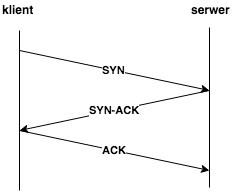
\includegraphics[height=8cm,keepaspectratio]{img/TCP_handshake.png}
    \caption{Schemat prezentujący trójstronne uzgodnienie (ang. \textit{three-way handshake}). Najpierw klient wysyła (chce zsynchronizować) swój numer sekwencji (SYN). Serwer odpowiada ACK (potwierdza udaną synchronizację) oraz SYN (synchronizacja własnego numeru sekwencji). Na końcu klient potwierdza synchronizację i może nastąpić transmisja właściwych danych.}
    \label{fig:TCP_handshake}
\end{figure}


\section{Gniazda dziedziny Uniksa}

Gniazda dziedziny Uniksa są podobne do zwykłych gniazd, jednak cała komunikacja zachodzi wewnątrz jądra systemu operacyjnego, zamiast korzystać z sieci. W tej metodzie komunikacji, system plików jest używany jako przestrzeń adresowa. Procesy traktują gniazda dziedziny Uniksa jako i-węzły (ang. \textit{i-nodes}), więc wiele procesów może komunikować się poprzez otwieranie tego samego gniazda.


\section{Systemy kolejkowe}

Systemy kolejkowe umożliwiają odłożenie wiadomości na kolejkę, z której weźmie ją odbiorca. Dzięki temu procesy nie muszą wchodzić w bezpośrednią interakcję. Cechy kolejek komunikatów zależne są od implementacji. Na przykład standard \textit{System V} posiada zarówno blokujące, jak i nieblokujące funkcje odbioru wiadomości. POSIX oferuje ponadto możliwość rejestracji funkcji odbierającej powiadomienie, która zostanie wywołana, kiedy pojawi się nowy komunikat. Dzięki temu odbiorca nie musi odpytywać kolejki (ang. \textit{polling}), marnując czas procesora, ani zatrzymywać wykonywania programu.


\section{Przekazywanie wiadomości}

Programy moga także komunikować się kanałami niezarządzanym przez system operacyjny. Wysyłana jest wiadomość, a za uruchomienie odpowiedniego kodu odpowiada odbiorca i infrastruktura wspomagająca. Ten sposób jest często używany do budowania rozproszonych aplikacji. Komunikacja może być zarówno synchroniczna, jak i asynchroniczna. Abtrakcją innego procesu może być obiekt, ale też na przykład aktor (np. stosowany w Akkce\cite{akka} model aktorów). Przesyłanie wiadomości może być zaimplementowane w dowolny sposób.


\subsection{Zdalne wykonywanie procedur}

Zdalne wykonywanie procedur (RPC - ang. \textit{remote procedure call}) to protokół utworzony przez firmę Sun\cite{rpc} i dość popularny w systemach z rodziny Unix. Służy do uruchomienia procedury w innej przestrzeni adresowej (zazwyczaj na innym komputerze w sieci). Wywołanie niczym nie różni się od lokalnych funkcji, ukrywając przed programistą szczegóły zdalnej komunikacji. Abstrakcja ta ułatwia tworzenie oprogramowania, jednak zawsze należy pamiętać, że uruchamianie kodu na innej maszynie niesie za sobą narzut komunikacyjny i nie należy go nadużywać.


\subsection{Java RMI}

Java RMI (ang. \textit{Java remote method invocation}) jest obiektowym odpowiednikiem RPC dla Javy. Technologia ta korzysta z serializacji Javy oraz rozproszonego odśmiecania pamięci (ang. \textit{distributed garbage collection}). Pozwala na zdalne wykonywanie metod na obiektach, które mogą znajdować się na innych maszynach wirtualnych Javy. Wymaganiem jest wcześniejsza rejestracja takich obiektów pod wybranymi nazwami w rejestrze \textit{RMI Registry}. Klient może pobrać tzw. \textit{stub}, czyli obiekt umożliwiający komunikację ze zdalną implementacją, mający taki sam interfejs. Wywoływanie metod jest idenetyczne jak w przypadku lokalnych obiektów. Rejestr nie pośredniczy w komunikacji. Wadą tej technologii jest brak wsparcia dla innych języków programowania.


\subsection{CORBA}

CORBA jest standardem zdefiniowanym przez OMG (ang. \textit{Object Management Group}) wydanym w 1991 roku \cite{CORBA}. Jego cel to umożliwienie komunikacji między procesami stworzonymi z użyciem innych języków programowania, na niezależnych maszynach - bez względu na sprzęt, czy system operacyjny. Wykorzystany został model obiektowy, mimo to języki programowania nie muszą wspierać paradygmatu obiektowego, aby używać technologii CORBA.

CORBA wprowadza warstwę abstrakcji, która ukrywa różnice pomiędzy systemami. Wykorzystuje język opisu interfejsu (IDL - ang. \textit{Interface Description Language}). Każdy język programowania kompiluje pliki IDL na kod zajmujący się przekazaniem metod, a w przypadku języków interpretowanych, IDL jest interpretowany w czasie wykonania. CORBA specyfikuje sposób mapowania IDL dla języków programowania takich jak np. C, C++, Java, Ada, COBOL, Lisp, Object Pascal, Python, Ruby czy Smalltalk. Zazwyczaj implementacja ORB (ang. \textit{Object Request Broker}) dostarcza kompilator IDL.


\begin{lstlisting}[caption={Przykład użycia IDL},captionpos=b]
    module ModuleExample {
        interface Math  {
            double sum(in double x, in double y);
        };
    };
\end{lstlisting}


Skorzystać możemy z wielu predefiniowanych typów (np. \textit{short}, \textit{long}, \textit{double}, \textit{string}), jak również tworzyć własne struktury czy unie oparte o typy elementarne.

W technologii CORBA istnieje jawny podział na klienty i serwery. Klient posiada interfejs pożądanego obiektu oraz jego implementację, która zostanie oddelegowana do serwera. Aby się z nim połączyć trzeba posiadać jego referencję - IOR (ang. \textit{Interoperable Object Reference}). Alternatywną jest skorzystanie z serwisu nazw (ang. \textit{NameService}) - działa on podobnie do systemu nazw domenowych (DNS). Serwer rejestruje się w nim pod wybraną nazwą, by klient mógł za jej pomocą uzyskać zarejestrowany IOR.

\begin{figure}[h]
    \centering
    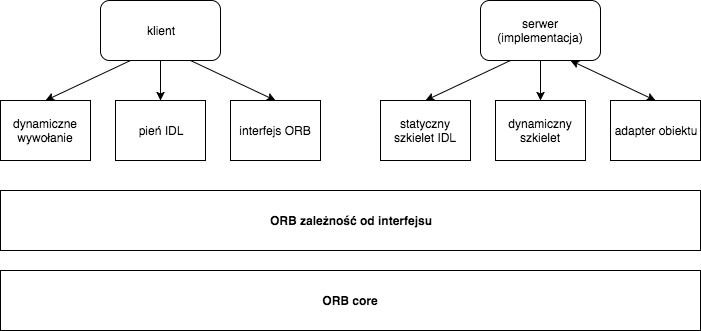
\includegraphics[width=\textwidth,height=\textheight,keepaspectratio]{img/CORBA_architecture.png}
    \caption{Schemat architektury aplikacji korzystającej z technologii CORBA \cite{Saw02}.}
    \label{fig:CORBA_architecture}
\end{figure}


\section{Java Native Interface}

Java Native Interface (JNI) co prawda nie jest metodą komunikacji między procesami, mimo to umożliwia integrację z programami napisanymi w innych językach. Pozwala, aby kod Javy uruchomiony w wirtualnej maszynie wywoływał oraz był wywoływany przez natywne aplikacje (napisane mogą one być w C, C++, asemblerze, ale także na przykład w Go i Rust) \cite{JNI17}.

Cel JNI to możliwość wykonania wszystkiego, co nie jest wykonalne używając jedynie Javy, np. wykorzystywywanie bibliotek zależnych od platformy oraz zwiększenie wydajności w krytycznych obszarach aplikacji.

Natywne programy mogą korzystać z obiektów Javy (tworzyć je, wykonywać metody, odbierać przekazane w parametrach). Sama biblioteka standardowa Javy wykorzystuje tę technologię.

\begin{table}[h!]
  \centering
  \begin{tabular}{|c|c|c|}
    \hline
    \textbf{Typ w Javie} & \textbf{Typ w JNI} & \textbf{Opis} \\ [0.5ex]
    \hline
    boolean & jboolean & 8 bitów bez znaku \\
    byte & jbyte & 8 bitów ze znakiem \\
    char & jchar & 16 bitów bez znaku \\
    short & jshort & 16 bitów ze znakiem \\
    int & jint & 32 bity ze znakiem \\
    long & jlong & 64 bity ze znakiem \\
    float & jfloat & 32 bity \\
    double & jdouble & 64 bity \\
    void & void & - \\ [1ex]
    \hline
  \end{tabular}
  \caption{Mapowania typów w JNI}
\end{table}


\section{REST}

REST jest stylem architektonicznym służącym do reprezentacji zasobów oraz ich manipulacji. Korzysta on z protokołu HTTP (sekcja \ref{HTTP_section}). Nie oferuje serwisów, które można wykorzystać, lecz zasoby, na których pozwala wykonywać akcje.

Wykorzystywane są metody HTTP, które wykonują akcje zgodne ze specyfikacją \cite{RFC7231}. Zasoby adresowane są za pomocą URI. REST nie jest protokołem, brakuje więc standardu jasno go opisującego. Formatem danych najczęściej jest JSON. Metody takie jak na przykład GET, PUT, DELETE są idempotentne, to znaczy, że wielokrotne ich wywołanie powoduje identyczny efekt jak jednokrotne.

Rozwinięciem jest HATEOAS (ang. \textit{Hypermedia As The Engine Of Application State}). Odpowiedzi serwera zwierają wtedy linki do innych zasobów, umożliwiając przejście wszystkich powiązań pomiędzy obiektami przez klienta. Analogicznie działają hiperłącza zamieszczone na stronach internetowych, dzięki czemu użytkownik może się nawigować znając tylko jeden adres.

\begin{table}[h!]
  \centering
  \begin{tabular}{|c|c|c|}
    \hline
    & \textbf{Pojedynczy zasób np.} & \textbf{Kolekcja np.} \\
    & \url{http://example.com/api/items/1} & \url{http://example.com/api/items} \\ [0.5ex]
    \hline
    \textbf{GET} & Zwraca reprezentację zasobu & Zwraca całą kolekcję \\
    \hline
    \textbf{POST} & Zazwyczaj nie używany & \begin{tabular}{@{}c@{}} Tworzy nowy zasób wykorzystując wysłany \\ przez klienta, zazwyczaj w odpowiedzi \\ znajduje się adres nowego elementu \end{tabular} \\
    \hline
    \textbf{PUT} & \begin{tabular}{@{}c@{}} Zamienia wybrany zasób \\ na wysłany przez klienta \end{tabular} & \begin{tabular}{@{}c@{}} Zamienia całą kolekcję \\ na wysłaną przez klienta \end{tabular} \\
    \hline
    \textbf{DELETE} & Usuwa zasób & Usuwa całą kolekcję \\
    \hline
  \end{tabular}
  \caption{Sposób działania przykładowych metod HTTP na zasobach}
\end{table}


\subsection{Protokół HTTP}

\label{HTTP_section}
HTTP (ang. \textit{Hypertext Transfer Protocol}) to bezstanowy protokół przesyłania dokumentów hipertekstowych w sieci WWW (ang. \textit{World Wide Web}). Do transportu wykorzystuje TCP. Jego działanie określić można jako zapytanie-odpowiedź. Klientem może być przeglądarka internetowa, która dokonuje żądań zasobów. Żądania te składają się z metody (np. GET, POST, HEAD, PUT, DELETE, OPTIONS) oraz Ujednoliconego Identyfikatora Zasobów (URI - ang. \textit{Uniform Resource Identifier}). W zapytaniu wysłane mogą być nagłówki (np. Accept, Content-Type, Host, Authorization). Metody takie jak POST, PUT umożliwiają wysłanie ciała zapytania (np. wiadomość w formacie JSON, XML). Odpowiedź od serwera także zawiera nagłówki i ciało, ale również kod statusu, który dostarcza dodatkowych informacji:
\begin{itemize}
  \item 1xx - kody informacyjne
  \item 2xx - kody powodzenia
  \item 3xx - kody przekierowania
  \item 4xx - kody błędu aplikacji klienta
  \item 5xx - kody błędu serwera HTTP
\end{itemize}


\begin{lstlisting}[caption={Przykład żądania HTTP},captionpos=b]
    GET /index.html HTTP/1.1
    Host: www.example.com
\end{lstlisting}

Serwer zwraca odpowiedź lub informuje o wystąpieniu błędu:

\begin{lstlisting}[caption={Przykład odpowiedzi serwera ze statusem 200 OK},captionpos=b]
    HTTP/1.1 200 OK
    Date: Mon, 11 May 2017 21:17:46 GMT
    Content-Type: text/html; charset=UTF-8
    Content-Encoding: UTF-8
    Content-Length: 138
    Last-Modified: Wed, 08 Jan 2003 23:11:55 GMT
    Server: Apache/1.3.3.7 (Unix) (Red-Hat/Linux)
    Connection: close

    <html>
        <head>
            <title>Przykładowy tytuł</title>
        </head>
        <body>
            Przykładowa odpowiedź
        </body>
    </html>
\end{lstlisting}


\section{SOAP}

SOAP (ang. \textit{Simple Object Access Protocol}) to protokół mający na celu tworzenie usług sieciowych, cechujących się uniezależnieniem od implementacji oraz platformy. Najczęściej korzysta z protokołu HTTP (sekcja \ref{HTTP_section}). Wiadomości transportowane są w formacie XML.

Obowiązuje je ścisła struktura, wiadomość składa się z \cite{SOAP}:
\begin{itemize}
    \item Envelope - identyfikuje dokument jako wiadomość SOAP
    \item Header - zawiera nagłówki, metadane
    \item Body - zawiera żądanie lub odpowiedź
    \item Fault - dostarcze informacje o błędach, jeśli zaszły w trakcie przetwarzania
\end{itemize}

\begin{lstlisting}[caption={Przykład zapytania, które jest zgodne z protokołem SOAP},captionpos=b]
    <?xml version="1.0" encoding="UTF-8"?>
    <soap:Envelope xmlns:soap="http://www.w3.org/2003/05/soap-envelope"
            xmlns:a="http://www.example.org/stocks">
        <soap:Header>
        </soap:Header>
        <soap:Body>
            <a:GetStockPrice>
                <a:StockName>COMPANY_NAME</a:StockName>
            </a:GetStockPrice>
        </soap:Body>
    </soap:Envelope>
\end{lstlisting}


\section{Porównanie wydajności potoków, pamięci współdzielonej oraz gniazda dziedziny Uniksa}

Porównując niskopoziomowe rozwiązania, ściśle powiązane z systemem operacyjnym dostrzec można pewną zależność \cite{ZX2011}:

\begin{itemize}
    \item dla danych mniejszych niż 4600 bajtów - pamięć współdzielona jest najszybsza
    \item dla danych między 5100 a 12000 bajtów - gniazdy dziedziny Uniksa okazały się najlepsze
    \item w pozostałych przypadkach zwyciężyły potoki nienazwane
\end{itemize}

\chapter{Implementacja}

Założeniem projektu było stworzenie konfigurowalnej platformy umożliwiającej przeprowadzanie testów wydajnościowych dla różnych metod komunikacji międzyprocesowej. Głowna część (silnik testujący) zrealizowana została w oparciu o Javę 9 i jej wirtualną maszynę.

Dane wejściowe to m. in. wybrany sposób komunikacji oraz jego konfiguracja, a także rozmiar danych do wysłania i odbioru. Aplikacja wykona pomiary oraz zapisze wyniki w formacie CSV.

Wartość, która jest istotna to czas jaki zajęła dwukierunkowa komunikacja. Cechuje się ona nanosekundową precyzją, lecz jej rozdzielczość jest większa. Wynika to działania metody \textit{System.nanoTime()} w Javie.

\begin{lstlisting}[caption={Metoda klasy abstrakcyjnej AbstractTransferTester, która jest wykorzysywana przez wszystkie sposoby komunikacji do wykonania pomiarów (implementowane/przeciążane są ostatnie 3 metody).},captionpos=b]
    public Metrics test(TestProps testProps) {
        beforeTest(testProps);
        long start = System.nanoTime();
        try {
            execute(testProps);
        } catch (TesterException e) {
            log.error("TesterException", e);
            afterTest();
            return Metrics.error(testProps.getRequestBytes().length,
                    testProps.getResponseSize(), testType);
        }

        long time = System.nanoTime() - start;
        afterTest();
        return Metrics.of(time, testProps.getRequestBytes().length,
                testProps.getResponseSize(), testType);
    }

    protected void beforeTest(TestProps testProps) {}

    protected abstract void execute(TestProps testProps) throws TesterException;

    protected void afterTest() {}
\end{lstlisting}


Aby zachować wiarygodność testów, przeprowadzone zostały wielokrotnie - każda wykorzystana konfiguracja testowa była wykonana co najmniej 1000-krotnie.

Przed właściwym testowaniem zawsze następowały uruchomienia niepomiarowe, aby \enquote{rozgrzać maszynę writualną}. To znaczy, aby uzyskać pełną wydajność. Celem jest wcześniejsze załadowanie klas do pamięci oraz poczekanie aż JIT (ang. \textit{just-in-time compilation} - kompilacja tuż przed wykonaniem kodu) dokona kompilacji do kodu natywnego oraz optymalizacji.

Charater testów był czysto naukowy. Dane przesyłane w zapytaniach to losowe bajty oraz rozmiar oczekiwanej odpowiedzi, aby dynamicznie sterować wielkościami komunikatów - bez rekonfigurowania serwerów oczekujących na klienta.

Odpowiedź generowana po stronie implementowanej w C/C++ została ujednolicona, tak aby nie fałszować różnic między metodami transportu.

\begin{lstlisting}[caption={Fragment kodu wykorzystywanego w każdej metodzie komunikacji do generowania odpowiedzi},captionpos=b]
    for (int i = 0; i < responseSize; i++) {
        response[i] = (i % 26) + 65;
    }
\end{lstlisting}

\begin{figure}[h!]
    \centering
    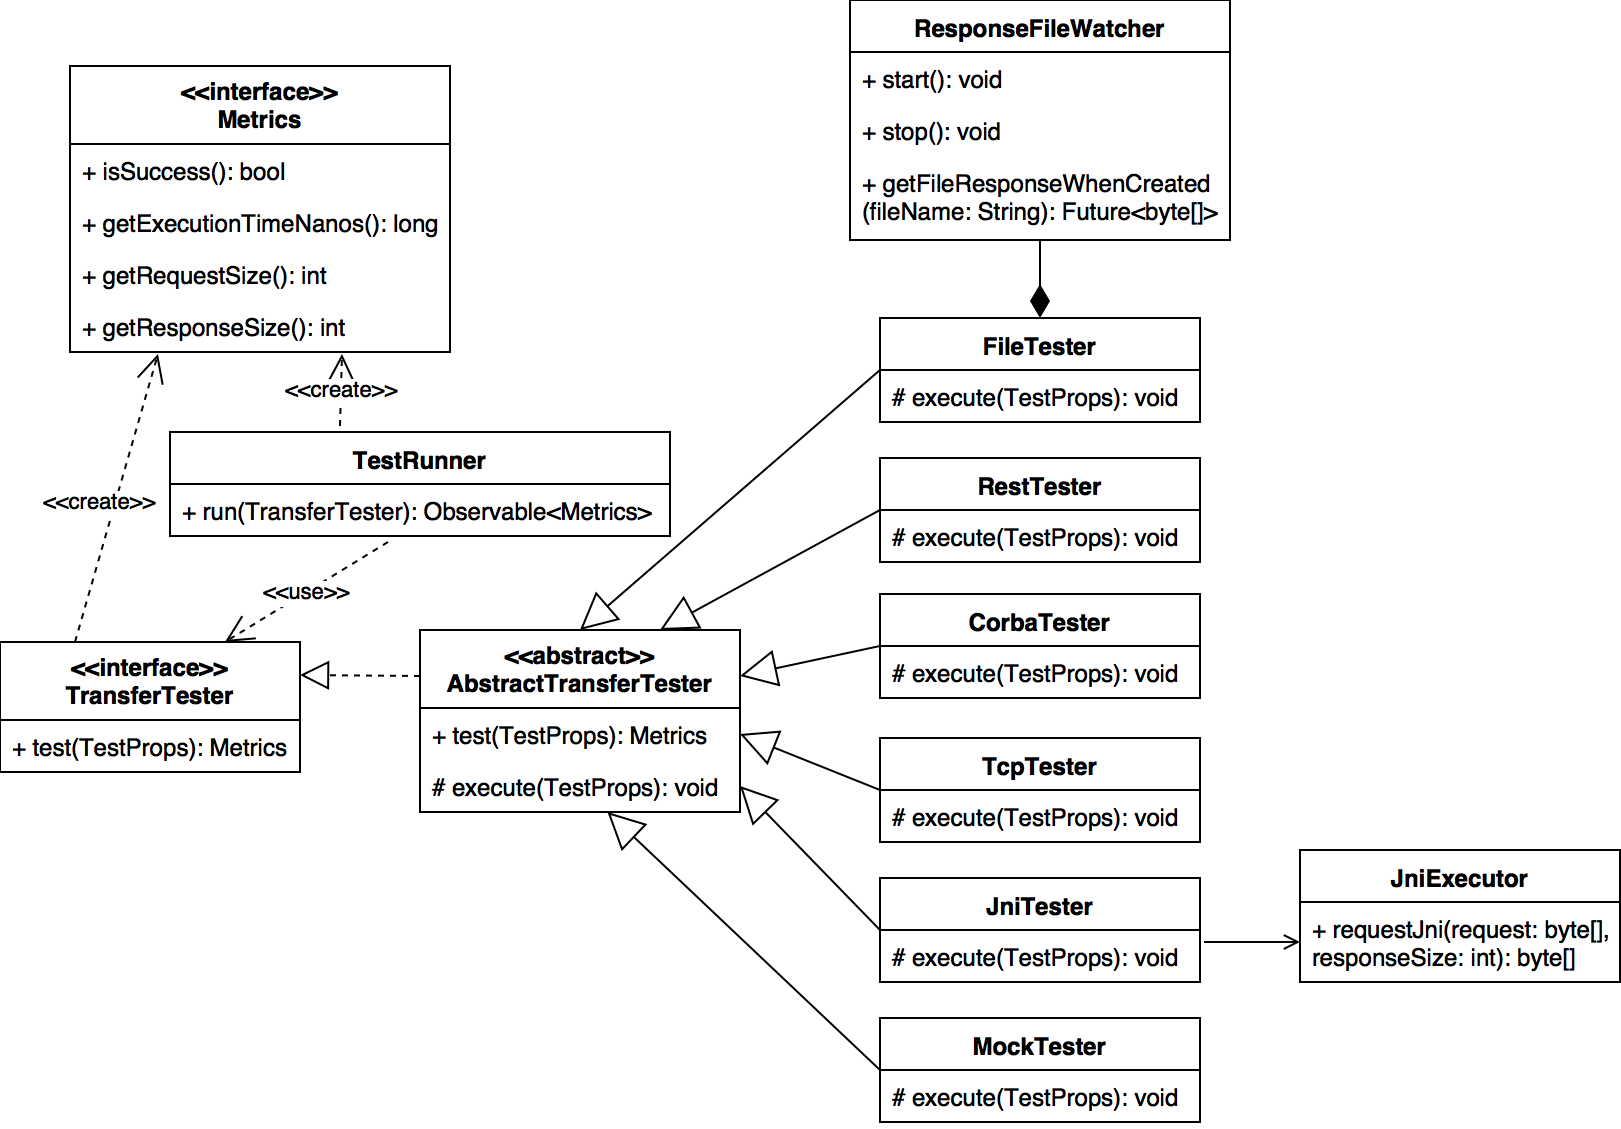
\includegraphics[width=\textwidth,height=\textheight,keepaspectratio]{img/class_diagram.png}
    \caption{Uproszczony diagram klas wykorzystany w silniku testującym.}
\end{figure}

W kolejnych sekcjach przybliżony zostanie sposób testowania poszczególnych metod komunikacji. Platformą docelową dla wszystkich implementacji jest Linux - na nim przeprowadzone zostały wszystkie uruchomienia (mimo że większość wspiera także macOS oraz Windows).

\section{Własny protokół oparty o TCP}

Zaimplementowany został własny protokół służący badaniu szybkości transferu danych oparty o gniazda TCP. Aby klient mógł zlokalizować serwer potrzebny jest mu jego adres IP i port oraz oczywiście musi istnieć możliwość stworzenia trasy.

Strona serwerowa wykorzystuje bibliotekę \texttt{unistd.h}. Klient opiera się o~standardową bibliotekę Javy, czyli klasę \texttt{java.net.Socket}.

\begin{figure}[h!]
    \centering
    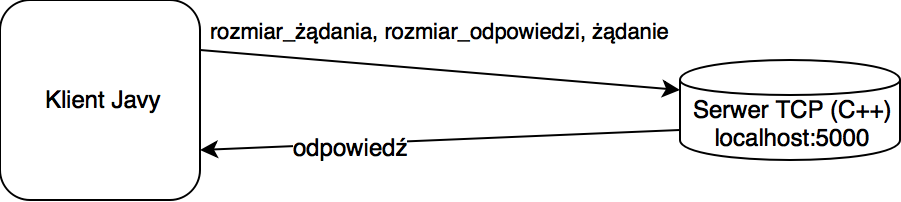
\includegraphics[width=\textwidth,height=\textheight,keepaspectratio]{img/tcp_impl_diagram.png}
    \caption{Diagram prezentujący działanie własnego protokołu opartego na TCP}
\end{figure}

Sam protokół należy do typu żądanie/odpowiedź - to znaczy za każdym razem otwierane jest gniazdo, a po otrzymaniu odpowiedzi zamykane. Jego działanie wygląda następująco:
\newline
Klient wysyła wiadomość składającą się kolejno z:
\begin{enumerate}
    \item 4 bajtów rozmiaru żądania
    \item 4 bajtów rozmiaru oczekiwanej odpowiedzi
    \item bajtów żądania w rozmiarze określonym na początku
\end{enumerate}
Serwer odpowiada bajtami odpowiedzi w rozmiarze określonym przez klienta (sam je generuje).


\section{REST}

Aby mogła zaistnieć komunikacja wykorzystująca REST, należało wcześniej wybrać format danych i~URI.

Serwer wystawia zasób pod adresem \texttt{/testResult}. Dane transferowane są w formacie JSON:
\begin{lstlisting}[caption={Format danych wysyłany przez klienta},captionpos=b]
    {
        "responseSize": 1024,
        "data": "ABCDEFGH..."
    }
\end{lstlisting}

\begin{lstlisting}[caption={Format danych zwracany przez serwer},captionpos=b]
    {
        "result": "ABCDEF..."
    }
\end{lstlisting}

\begin{figure}[h!]
    \centering
    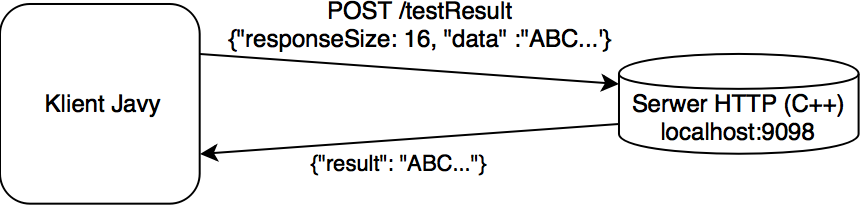
\includegraphics[width=\textwidth,height=\textheight,keepaspectratio]{img/rest_impl_diagram.png}
    \caption{Diagram prezentujący komunikację klienta z serwerem HTTP}
\end{figure}

Implemetancja strony serwerowej wykorzystuje bibliotekę ngrest (\url{https://github.com/loentar/ngrest}), służącą do tworzenie serwisów RESTowych.

Klient Javy oparty jest \textit{OkHttp} (\url{http://square.github.io/okhttp}) jako klienta HTTP oraz \textit{Jackson} \newline (\url{https://github.com/FasterXML/jackson}) do parsowania i budowania formatu JSON.


\section{Pliki}

System plików nie został stworzony w celu komunikacji typu żądanie-odpowiedź. Należało zatem zaimitować takie zachowanie. Został zaimplementowany własny protokół, który spełnia taką funkcję.

Format pliku żądania zawiera:
\newline
\texttt{rozmiar\_oczekiwanej\_odpowiedzi, bajty\_zapytania}

Rozmiar oczekiwanej odpowiedzi to 4 bajty (liczba całkowita). Plik zwrotny zawiera jedynie bajty z odpowiedzią.

Poniżej znajduje się diagram przedstawiający komunikację.

\begin{figure}[h!]
    \centering
    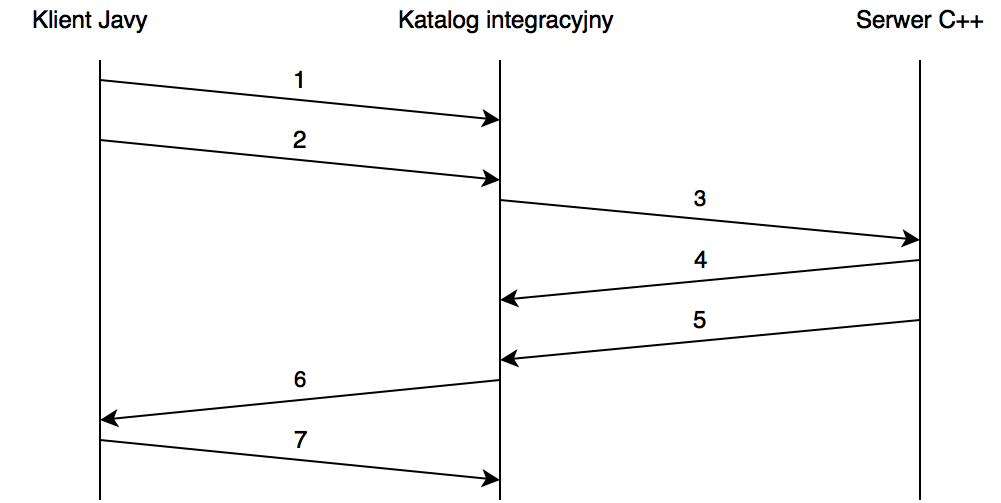
\includegraphics[width=\textwidth,height=\textheight,keepaspectratio]{img/files_impl_diagram.png}
    \caption{}
\end{figure}

\texttt{UUID} w poniższym opisie oznacza losowy ciąg znaków generowany po stronie klienta.
\begin{enumerate}
    \item Stworzenie pliku o nazwie \texttt{UUID\_request\_tmp} i zapisanie w nim żądania w formacie: 4 bajty dla rozmiaru oczekiwanej odpowiedzi, bajty żądania
    \item Zmiana nazwy stworzonego pliku na \texttt{UUID\_request}
    \item Wczytanie pliku, którego nazwa kończy się na \texttt{\_request}
    \item Stworzenie pliku o nazwie \texttt{UUID\_response\_tmp} i zapisanie w nim odpowiedzi (w żądanym rozmiarze)
    \item Zmiana nazwy pliku na \texttt{UUID\_response}
    \item Wczytanie odpowiedzi z pliku \texttt{UUID\_response}
    \item Usunięcie plików \texttt{UUID\_request} i \texttt{UUID\_response}
\end{enumerate}

W kliencie Javy zastosowany został komponent \textit{File Monitor} z biblioteki \textit{Apache Commons IO} (\url{https://commons.apache.org/proper/commons-io}). Niestety nie wspiera on natywnych interfejsów informujących o zdarzeniach w systemie plików (np. \textit{inotify} dla Linuksa, FSEvents dla macOS, czy \textit{FileSystemWatcher} dla Windowsa). Zamiast tego skonfigurowne zostało skanowanie katalogu co 2ms.

Serwer C++ wykorzystuje \textit{inotify} (podsystem jądra Linuksa, który służy do powiadamia o zdarzeniach w systemie plików \cite{inotify_man}), dzięki czemu implementacja jest wydajna i nie wykonuje zbędynch skanów katalogu.


\section{CORBA}

Aplikacje, które należy zintegrować opierając się na specyfikacji Corby, muszą skorzystać z wybranej implementacji. OmniORB jest jedną z bardziej popularnych i wydajnych. Została użyta w wersji 4 przez serwer C++. Klient wykorzystuje zaś tę dołączoną do Javy 9.

Komunikacja pomija serwis nazw - klient zna IOR, do którego wysyła zapytania.

\begin{lstlisting}[caption={Zastosowany interfejs (IDL)},captionpos=b]
    module pl {
        module kumon {
            module transfertester {
                module tester {
                    module corba {

                        interface CorbaConnector {
                            string get(in long responseSize, in string request);
                        };
                    };
                };
            };
        };
    };
\end{lstlisting}

Protokół wymiany danych informuje serwer, jakej długości jest oczekiwana odpowiedź oraz przekazuje samo żądanie. Informacja zwrotna zostaje wygenerowana tak, aby dotrzymać wymaganego rozmiaru.


\section{JNI}

Java Native Interface wymaga stworzenia pomostu między maszyną wirtualną Javy a kodem natywnym. Stworzony został interfejs komunikacji.

\begin{lstlisting}[caption={Metoda javy, która wymaga natywnej implementacji.},captionpos=b]
    public class JniExecutor {
        public native byte[] requestJni(byte[] requestBytes, int responseSize);
    }
\end{lstlisting}

Implementacja w C żądanie i oczekiwaną długość odpowiedzi, jednak są to struktury typów \texttt{jbyteArray} i \texttt{jint}, więc przed użyciem wymagają odpowiedniego mapowania. Podobnie wygląda generowanie danych zwrotnych - oczekiwany typ to \texttt{jbyteArray}.

\begin{lstlisting}[caption={Natywna implementacja w C.},captionpos=b]
    JNIEXPORT jbyteArray JNICALL Java_pl_kumon_transfertester_tester_jni_JniExecutor_requestJni(
    JNIEnv *env, jobject thisObj, jbyteArray requestBytes, jint responseSize) {

        readRequest(env, &requestBytes);
        jbyteArray response = (*env)->NewByteArray(env, responseSize);
        jbyte *bytes = prepareResponseRandomBytes(env, &response, responseSize);
        (*env)->SetByteArrayRegion(env, response, 0, responseSize, bytes);
        return response;
    }

    void readRequest(JNIEnv *env, jbyteArray* requestBytes) {
        unsigned char* buffer = (*env)->GetByteArrayElements(env, *requestBytes, NULL);
        jsize size = (*env)->GetArrayLength(env, *requestBytes);
        (*env)->ReleaseByteArrayElements(env, *requestBytes, buffer, JNI_ABORT);
    }

    jbyte* prepareResponseRandomBytes(JNIEnv *env, jbyteArray *response, jint responseSize) {
        int i;
        jbyte *bytes = (*env)->GetByteArrayElements(env, *response, 0);
        for (i = 0; i < responseSize; i++) {
            bytes[i] = (i % 26) + 65;
        }
        return bytes;
    }
\end{lstlisting}


\section{Implementacja bez komunikacji}

Ciekawy do sprawdzenia jest sam narzut platofrmy testowej, który nie wynika z generowania odpowiedzi. Aby tego dokonać, stworzony został test działający jedynie w pamięci wirtualnej maszyny Javy, który nie komunikuje się z niczym na zewnątrz.

Uniknięcie optymalizacji (aby cała pętla nie została pominięta) zostało osiągnięte przez kontrolę rozmiaru wygenerowanych danych.

\begin{lstlisting}[caption={Test sprawdzający narzut samej platformy.},captionpos=b]
    protected void execute(TestProps testProps) throws TesterException {
        byte[] mockResponse = getMockResponse(testProps.getResponseSize());
        ResponseValidator.validateLength(mockResponse, testProps);
    }

    private byte[] getMockResponse(int responseSize) {
        byte[] response = new byte[responseSize];
        for (int i = 0; i < responseSize; i++) {
            response[i] = (byte) ((i % 26) + 65);
        }
        return response;
    }
\end{lstlisting}

\chapter{Prezentacja wyników}

Przeprowadzone zostały testy dla zaimplementowanych metod komunikacji. Wszystkie miały charakter lokalny (transmisja sieciowa wykorzystywała \textit{localhost}). Sprawdzone zostały różne rozmiary żądań i odpowiedzi w wielu kombinacjach (16B - 128MiB). Generowanie danych opisane zostało w rozdziale \ref{data_generation}.

Wszystkie uruchomienia korzystały z tej samej platformy:
\begin{itemize}
    \item System operacyjny: Ubuntu 17.10
    \item Java 9.0.1+11
    \item Procesor: intel i5 4690k
    \item Pamięć RAM: 16GB 2400MHz CL10
    \item dysk SSD (odczyt 250 MB/s, zapis 500MB/s, 72000 IOPS)
\end{itemize}


\section{Rozkład danych}

Każda konfiguracja testowa wykonana została co najmniej 1000-krotnie. Z otrzymanych wyników obliczona została średnia arytmetyczna oraz odchylenie standardowe, ponieważ ich wykresy zbliżone są rozkładu normalnego. Poniżej znajdą się diagramy, które to ukazują (dla wybranych metod).

\vspace{5mm} 

\pgfmathdeclarefunction{gauss}{2}{%
    \pgfmathparse{1/(#2*sqrt(2*pi))*exp(-((x-#1)^2)/(2*#2^2))}%
}

\begin{tikzpicture}
\begin{axis}[
    height=7.5cm,
    width=15cm,
    grid=major,
    ylabel={Wystąpienia w przedziale},
    xlabel={Czas wykonania [$\mu$s]},
    legend style={cells={align=right}}
]

\addplot[draw=blue] coordinates {
    (255,0)
    (260,0)
    (265,0)
    (270,10)
    (275,13)
    (280,22)
    (285,23)
    (290,21)
    (295,20)
    (300,31)
    (305,22)
    (310,31)
    (315,33)
    (320,35)
    (325,37)
    (330,29)
    (335,37)
    (340,35)
    (345,35)
    (350,49)
    (355,33)
    (360,22)
    (365,29)
    (370,24)
    (375,30)
    (380,17)
    (385,31)
    (390,20)
    (395,20)
    (400,19)
    (405,18)
    (410,17)
    (415,18)
    (420,26)
    (425,12)
    (430,10)
    (435,9)
    (440,12)
    (445,10)
    (450,11)
    (455,8)
};
\addlegendentry{TCP - żądanie 8KiB,\\odpowiedź 8KiB}

\addplot[domain={255:455},yscale=4500,samples=150] {gauss(352,46)};

\end{axis}
\end{tikzpicture}


\begin{tikzpicture}
\begin{axis}[
    height=8cm,
    width=15cm,
    grid=major,
    ylabel={Wystąpienia w przedziale},
    xlabel={Czas wykonania [$\mu$s]},
    legend style={cells={align=right}}
]

\addplot[draw=blue] coordinates {
    (2303,0)
    (2319,0)
    (2335,0)
    (2351,0)
    (2367,0)
    (2383,0)
    (2399,7)
    (2415,19)
    (2431,15)
    (2447,14)
    (2463,6)
    (2479,7)
    (2495,22)
    (2511,15)
    (2527,31)
    (2543,20)
    (2559,31)
    (2575,39)
    (2591,41)
    (2607,40)
    (2623,47)
    (2639,48)
    (2655,50)
    (2671,43)
    (2687,49)
    (2703,45)
    (2719,51)
    (2735,41)
    (2751,42)
    (2767,36)
    (2783,23)
    (2799,27)
    (2815,22)
    (2831,14)
    (2847,7)
    (2863,9)
    (2879,5)
    (2895,4)
    (2911,3)
    (2927,1)
    (2943,2)
};
\addlegendentry{Pliki - żądanie 1MiB,\\odpowiedź 16B}

\addplot[domain={2303:2943},yscale=13800,samples=150] {gauss(2653,111)};

\end{axis}
\end{tikzpicture}


\begin{tikzpicture}
\begin{axis}[
    height=8cm,
    width=15cm,
    grid=major,
    ylabel={Wystąpienia w przedziale},
    xlabel={Czas wykonania [$\mu$s]},
    legend style={cells={align=right}}
]

\addplot[draw=blue] coordinates {
    (1636,0)
    (1651,0)
    (1666,3)
    (1681,6)
    (1696,14)
    (1711,15)
    (1726,15)
    (1741,17)
    (1756,27)
    (1771,30)
    (1786,29)
    (1801,29)
    (1816,35)
    (1831,36)
    (1846,30)
    (1861,44)
    (1876,33)
    (1891,30)
    (1906,43)
    (1921,46)
    (1936,35)
    (1951,36)
    (1966,25)
    (1981,32)
    (1996,29)
    (2011,36)
    (2026,15)
    (2041,20)
    (2056,20)
    (2071,30)
    (2086,21)
    (2101,14)
    (2116,13)
    (2131,21)
    (2146,17)
    (2161,12)
    (2176,8)
    (2191,12)
    (2206,9)
    (2221,10)
    (2236,3)
};
\addlegendentry{REST - żądanie 16B,\\odpowiedź 1KiB}

\addplot[domain={1636:2236},yscale=15000,samples=150] {gauss(1928,133)};

\end{axis}
\end{tikzpicture}


\section{Porównanie wyników}

Najważniejszym zestawieniem jest porównanie czasów komunikacji dla różnych kanałów transmisji danych, przy takim samym rozmiarze przesyłanych danych. Poniżej zaprezentowane zostaną przykładowe wykresy, zawierające średnie arytmetyczne oraz odchylenia standardowe. Wartości dla \textit{Mock} oznaczają implementację, która nie transmituje danych, tylko od razu je zwraca.


\begin{figure}[H]
\begin{tikzpicture}
\begin{axis}[
    title = {Żądanie 1KiB, odpowiedź 1KiB},
    width=15cm,
    height=10cm,
    xtick={1,...,7},
    xticklabels={
        CORBA,
        Pliki,
        Pliki (ramdysk),
        JNI,
        Mock,
        REST,
        TCP
    },
    ymin=0,
    ylabel={średnia [$\mu$s]},
    nodes near coords,
    grid=major,
    ybar
]
\addplot[
    fill=blue!25,
    draw=black,
    point meta=y,
    every node near coord/.style={inner ysep=5pt},
    error bars/.cd,
    y dir=both,
    y explicit
]
table [y error=error] {
    x       y        error     label
    1   1177     1435      1
    2   2571     1151      2
    3   2495     1342      3
    4   12         283        4
    5   6           168        5
    6   1501     176        6
    7   343       88          7
};
\end{axis}
\end{tikzpicture}
\caption{}
\label{fig:chart_1024_1024}
\end{figure}


Większość porównań dla innych rozmiarów danych jest proporcjonalna do wykresu \ref{fig:chart_1024_1024}. Pierwsze wnioski ukazują, że komunikacja przez pliki jest najwolniejsza, zdecydowanie najlepiej sprawuje się JNI, TCP prezentuje wysoką wydajność, a CORBA oraz REST mają wartości pośrednie.

\begin{figure}[H]
\begin{tikzpicture}
\begin{axis}[
    title = {Żądanie 16B, odpowiedź 1MiB},
    width=15cm,
    height=8cm,
    xtick={1,...,7},
    xticklabels={
        CORBA,
        Pliki,
        Pliki (ramdysk),
        JNI,
        Mock,
        REST,
        TCP
    },
    ymin=0,
    ylabel={średnia [$\mu$s]},
    nodes near coords,
    grid=major,
    ybar
]
\addplot[
    fill=blue!25,
    draw=black,
    point meta=y,
    every node near coord/.style={inner ysep=5pt},
    error bars/.cd,
    y dir=both,
    y explicit
]
table [y error=error] {
    x       y        error     label
    1   5586     1553      1
    2   3854     1380      2
    3   3176     1661      3
    4   381       317        4
    5   101       263        5
    6   13979   2194      6
    7   1976     660        7
};
\end{axis}
\end{tikzpicture}
\caption{}
\label{fig:chart_16_1048576}
\end{figure}

\begin{figure}[H]
\begin{tikzpicture}
\begin{axis}[
    title = {Żądanie 1MiB, odpowiedź 16B},
    width=15cm,
    height=8cm,
    xtick={1,...,7},
    xticklabels={
        CORBA,
        Pliki,
        Pliki (ramdysk),
        JNI,
        Mock,
        REST,
        TCP
    },
    ymin=0,
    ylabel={średnia [$\mu$s]},
    nodes near coords,
    grid=major,
    ybar
]
\addplot[
    fill=blue!25,
    draw=black,
    point meta=y,
    every node near coord/.style={inner ysep=5pt},
    error bars/.cd,
    y dir=both,
    y explicit
]
table [y error=error] {
    x       y        error     label
    1   5459     1240      1
    2   2834     1233      2
    3   2637     1549      3
    4   71         104        4
    5   3           94          5
    6   64170   9701      6
    7   1146     200        7
};
\end{axis}
\end{tikzpicture}
\caption{}
\label{fig:chart_1048576_16}
\end{figure}


Wykresy \ref{fig:chart_16_1048576} i \ref{fig:chart_1048576_16} prezentują różnicę w przypadku dużych zapytań lub odpowiedzi. Należy pamiętać, że czas alokowania pamięci dla wiadomości zwrotnej wlicza się do czasu komunikacji, więc te liczby nie mogą być równe. Różne pomiary mogą wynikać także z samych implementacji w innych technologiach (Java i C++), które inaczej reagują na rozmiary danych.
Dostrzec można również wielką dysproporcję w przypadku RESTa - prawdopodobnie wynika z niewydajnej implementacji biblioteki użytej po stronie serwera (sekcja \ref{REST_impl}). 

\begin{figure}[H]
\begin{tikzpicture}
\begin{axis}[
    title = {Żądanie 16B, odpowiedź 16B},
    width=15cm,
    height=8cm,
    xtick={1,...,7},
    xticklabels={
        CORBA,
        Pliki,
        Pliki (ramdysk),
        JNI,
        Mock,
        REST,
        TCP
    },
    ymin=0,
    ylabel={średnia [$\mu$s]},
    nodes near coords,
    grid=major,
    ybar
]
\addplot[
    fill=blue!25,
    draw=black,
    point meta=y,
    every node near coord/.style={inner ysep=5pt},
    error bars/.cd,
    y dir=both,
    y explicit
]
table [y error=error] {
    x       y        error     label
    1   1224     1486      1
    2   2579     1273      2
    3   2498     1763      3
    4   6.5        144        4
    5   3.7        100        5
    6   1496     269        6
    7   339       73          7
};
\end{axis}
\end{tikzpicture}
\caption{}
\label{fig:chart_16_16}
\end{figure}


Narzut wynikający z samej technologii przy minimalnych rozmiarach danych (16B - wykres \ref{fig:chart_16_16}) jest największy dla plików (wynika z obserwatora katalogu, który wykonuje skanowanie co 2ms). Wysoki okazuje się także dla RESTa (protokół HTTP oraz serializacja do formatu JSON). Sam mechanizm, którego używa CORBA, pochłania trochę ponad 1ms. Własny, bardzo prosty protokół oparty na TCP wykazuje wysoką wydajność gniazd. Jednak najszybsze jest wykonanie kodu natywnego przez wirtualną maszynę javy - cechuje się marginalnie niskim narzutem.
 

\begin{figure}[H]
\begin{tikzpicture}
\begin{axis}[
    title = {Żądanie 128MiB, odpowiedź 128MiB},
    width=15cm,
    height=8cm,
    xtick={1,...,7},
    xticklabels={
        Pliki,
        Pliki (ramdysk),
        JNI,
        Mock,
        TCP
    },
    ymin=0,
    ylabel={średnia [$ms$]},
    nodes near coords,
    grid=major,
    ybar
]
\addplot[
    fill=blue!25,
    draw=black,
    point meta=y,
    every node near coord/.style={inner ysep=5pt},
    error bars/.cd,
    y dir=both,
    y explicit
]
table [y error=error] {
    x       y        error     label
    1   259.1     1.98      1
    2   215        2.9        2
    3   97.57     1.6        3
    4   6.18       1.2        4
    5   89.86     1.6        5
};
\end{axis}
\end{tikzpicture}
\caption{}
\label{fig:chart_134217728_134217728}
\end{figure}

Testy zostały wykonane także dla dużych zestawów danych (128MiB - wykres \ref{fig:chart_134217728_134217728}). Im większe komunikaty tym stabilniejszy jest sam czas (znacznie niższe odchylenie standardowe). Ciekawe jest to, że komunikacja przez gniazda trwała krócej niż przez Java Native Interface.

Najstabilniejszą metodą transportu jest TCP - tam odchylenie standardowe okazuje się zwykle najniższe bezwzględnie lub w stosunku do samego czasu. W przypadku JNI wyniki mogą być bardzo rozrzucone, większość bardzo niska, ale zdarzają się kilkadziesiąt razy wolniejsze wykonania.
CORBA uzyskuje jedno z największych odchyleń standardowych, a pliki niewiele niższe. Jednak wraz ze wzrostem ilości przesyłanych danych, spada stosunek odchylenia standardowego do średniej, czyli transmisja stabilizuje się.

Implementacja testowa (bez transportu danych) zgodnie z przewidywaniami okazała się najszybsza. Udowadnia, że nie ma darmowej komunikacji. Każda generuje pewien narzut, więc nie zawsze warto delegować wykonanie do innych procesów.


\section{Tabela pomiarów}

Poniżej zaprezentowana została tabela (\ref{tab:all_results}) z zebranymi pomiarami. Zawiera średnie czasy wykonania dla różnych metod oraz współczynnik porównujący ilokrotnie różnią się dane względem JNI.

\begin{longtable}{|c|c|c|c|c|c|c|}
    \hline
    \begin{tabular}{@{}c@{}} \textbf{Rozmiar} \\ \textbf{zapytania} \end{tabular} & \begin{tabular}{@{}c@{}} \textbf{Rozmiar} \\ \textbf{odpowiedzi} \end{tabular} & \textbf{CORBA} [$\mu$s] & \textbf{Pliki} [$\mu$s] & \textbf{JNI} [$\mu$s] & \textbf{REST} [$\mu$s] & \textbf{TCP} [$\mu$s] \\
    \hline
    16B & 16B & 1224 (187.2x) & 2579 (394.4x) & 6.5 (1x) & 1496 (228.7x) & 338.9 (51.8x) \\
    16B & 1KiB & 1207 (235.6x) & 2578 (503.3x) & 5.1 (1x) & 1936 (377.9x) & 340 (66.4x) \\
    16B & 8KiB & 1179 (119x) & 2588 (261.2x) & 9.9 (1x) & 2089 (210.9x) & 349.4 (35.3x) \\
    16B & 256KiB & 2449 (14.7x) & 2978 (17.9x) & 166.5 (1x) & 6382 (38.3x) & 919.4 (5.5x) \\
    16B & 1MiB & 5586 (14.7x) & 3854 (10.1x) & 381.1 (1x) & 13979 (36.7x) & 1976 (5.2x) \\
    1KiB & 16B & 1147 (237.5x) & 2566 (531.2x) & 4.8 (1x) & 1983 (410.5x) & 351.5 (72.8x) \\
    1KiB & 1KiB & 1177 (97.1x) & 2571 (212.2x) & 12.1 (1x) & 1501 (123.8x) & 343.3 (28.3x) \\
    8KiB & 16B & 1324 (271.7x) & 2594 (532.3x) & 4.9 (1x) & 44126 (9055.3x) & 344.2 (70.6x) \\
    8KiB & 8KiB & 1319 (106.7x) & 2600 (210.3x) & 12.4 (1x) & 43997 (3559x) & 358.1 (29x) \\
    256KiB & 16B & 2385 (128.1x) & 2639 (141.8x) & 18.6 (1x) & 38275 (2056.2x) & 593.2 (31.9x) \\
    256KiB & 256KiB & 3199 (19.5x) & 3053 (18.6x) & 163.8 (1x) & 38627 (235.8x) & 1107 (6.8x) \\
    1MiB & 16B & 5459 (76.9x) & 2834 (39.9x) & 70.9 (1x) & 64170 (904.5x) & 1146 (16.2x) \\
    1MiB & 1MiB & 7728 (16.3x) & 4326 (9.2x) & 472.8 (1x) & 70718 (149.6x) & 2597 (5.5x) \\
    128MiB & 128MiB & - & 259100 (2.7x) & 97565 (1x) & - & 89859 (0.9x) \\
    \hline
    \caption{Tabela uzyskanych średnich czasów komunikacji wraz z porównaniem do JNI wykorzystując współczynnik.}
    \label{tab:all_results}
\end{longtable}


Dostrzec można, że wyniki nie skalują się liniowo wraz ze wzrostem transmitowanych danych. Porównując 2 ostatnie wiersze tabeli (1MiB i 128MiB) widać, że JNI nie został stworzony w celu przekazywania większych obiektów - rezultaty zmieniają się gorzej niż liniowo. Inaczej jest dla plików i TCP - tam bardziej opłaca się przesyłać większe dane naraz, ponieważ czasy nie zwolniły 128-krotnie a odpowiednio 60 i 35-krotnie.

\chapter{Podsumowanie}

Celem pracy było porównanie mechanizmów do współdzielenia danych między programami w języku Java i C/C++. Przeprowadzone testy pozwalają wyciągnąć kilka wniosków.
Java Native Interface okazuje się najszybszą metodą przekazywania danych do aplikacji natywnych. Cechuje się też stabilnością (niskie bezwzględne odchylenie standardowe - choć wysokie względem samego czasu). Nie pozwala jednak na wywołanie zdalne, a jedynie na lokalne, synchroniczne wykonanie metody. Nie ma więc do czynienia z delegowaniem wykonania do innego procesu, a jedynie uruchomieniem skompilowanej funkcji.

Bardziej uniwersalnym wyborem jest własny protokół oparty o TCP. Oferuje najwyższą wydajność przy transporcie informacji między już istniejącymi procesami. Dodatkowo komunikacja może być zarówno lokalna, jak i sieciowa. Niestety stosowanie własnego protokołu bywa uciążliwe. Należy go dobrze zdefiniować i wszędzie poprawnie zaimplementować. Znacznie łatwiej wykorzystać istniejące standardy.

Alternatywą jest CORBA. Otrzymujemy IDL oraz gotowe implementacje w zamian za niewielki narzut wydajnościowy. Podobnie w przypadku RESTa - można wykorzystać na przykład \textit{JSON Schema} (\url{http://json-schema.org}) do opisania interfejsów i biblioteki, które obsłużą całą warstwę transportową.

Wykorzystywanie systemu plików do komunikacji to dobry pomysł tylko w specjalnych przypadkach. Nie został on stworzony do wykonywania zapytań zachowując, mimo że to takie efekt jest osiągalny. Wyniki potwierdzają, że integracja przez pliki jest niewydajna, choć dla bardzo dużych danych (powyżej 100MB) warto ją rozważyć.


\section{Propozycje rozwoju}

W pracy przedstawione zostało porównanie 5 metod komunikacji. Dobrym pomysłem byłoby dodanie kolejnych sposobów przesyłania danych, np. protokół SOAP lub systemy pośredniczące w przesyłaniu wiadomości takie jak ActiveMQ (\url{http://activemq.apache.org}). Pozwoliłoby to uzyskać szerszy przegląd istniejących technologii.

Warto byłoby też przetestować inną implementację serwera REST dla C++. Użyta w pracy nie sprawdza się dla większych komunikatów.


% itd.
% \appendix
% \include{dodatekA}
% \include{dodatekB}
% itd.

\printbibliography

\end{document}
